\subsection{Queue Manager}\label{comp:queueManager}
\subsubsection{Internal Components}
The Queue Manager is responsible for the management of available taxi drivers, to store and retrieve them when asked and apply the policy decided. Internally it is composed of the following components each with a precise job:
\begin{itemize}
	\item \textit{ManagementLogic}: it is the component which apply the decided policy over available taxi drivers. It exposes general methods such as add remove and get in order to hide the internal management. Before any operation it retrieve the corresponding queue from the QueuesContainer and then it makes the necessary operation on the queue.
	\item \textit{QueueContainer}: as the name suggests, it is the container of the queues. It keeps then in a map with the zone as the key. It provide the ManagementLogic the methods for creating a queue or retrieving it.
\end{itemize}
\begin{figure}[H]
	\centering
	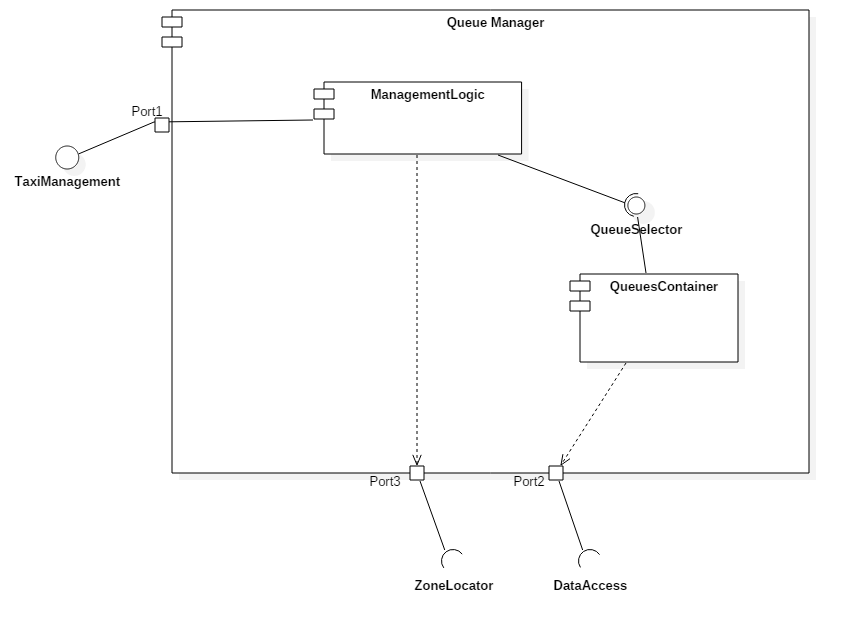
\includegraphics[scale=0.5]{../"Analysis Documents"/components/queueManager}
	\label{fig:queuemanager}
	\caption{Queue Manager internal structure}
\end{figure}
\subsubsection{Provided interfaces}
\begin{table}[H]
	\begin{longtable}{| p{0.3\textwidth} | p{0.3\textwidth} | p{0.4\textwidth} |}
		\hline
		\textbf{Provided Interface} & \textbf{Dedicated user} & \textbf{Description} \\ \hline
		TaxiManagement & Taxi Manager component & Provides the methods for adding, removing and retrieving taxi drivers to the data structure (queue) \\ \hline
	\end{longtable}
	\caption{Queue Manager: provided interfaces}
	\label{tab:queuemanager:providedInterfaces}
\end{table}
\subsubsection{Required interfaces}
\begin{table}[H]
	\begin{longtable}{| l | p{.80\textwidth} |}
		\hline
		\textbf{Required Interface} & \textbf{Description and usage} \\ \hline
		Zone Locator & Gets the list of the zones at the start up of the system in order to create the needed queues \\ \hline
		Data Access & Maintains the queues in the database \\ \hline
	\end{longtable}
	\caption{Queue Manager: required interfaces}
	\label{tab:queuemanager:requiredInterfaces}
\end{table}
